\documentclass[11pt]{article}
% Shared preamble for the course handouts and the cheatsheet (article class).
\usepackage[T1]{fontenc}
\usepackage[utf8]{inputenc}
\usepackage{lmodern}
\usepackage[a4paper, margin=2cm]{geometry}
\usepackage{amsmath, amssymb, bm, booktabs, graphicx, xcolor, enumitem, tcolorbox, multicol, listings}
\usepackage{tikz}
\usetikzlibrary{arrows.meta, positioning, calc}
\usepackage[hidelinks]{hyperref}
\setlength{\parindent}{0pt}
\setlength{\parskip}{0.5em}

% same colours and macros as the slides (slides/preamble.tex)
\definecolor{accent}{HTML}{C0392B}
\definecolor{cool}{HTML}{2E6DB4}
\definecolor{muted}{HTML}{7A7A7A}
\definecolor{good}{HTML}{2E8B57}
\definecolor{prob}{HTML}{E67E22}
\newcommand{\given}{\,|\,}
\newcommand{\E}{\mathbb{E}}
\newcommand{\KL}[2]{D_{\mathrm{KL}}\!\left[#1\,\middle\|\,#2\right]}
\newcommand{\N}{\mathcal{N}}
\newcommand{\Hess}{\mathcal{H}}
\DeclareMathOperator*{\argmin}{arg\,min}

% boxes
\newtcolorbox{keyidea}{colback=accent!5, colframe=accent!70!black, boxrule=0.6pt, arc=2pt, left=6pt, right=6pt, top=4pt, bottom=4pt}
\newtcolorbox{labhelp}[1]{colback=good!5, colframe=good!60!black, boxrule=0.6pt, arc=2pt, title={\small\bfseries #1}, fonttitle=\small, left=6pt, right=6pt, top=4pt, bottom=4pt}
\newtcolorbox{backupbox}[1]{colback=cool!5, colframe=cool!70!black, boxrule=0.6pt, arc=2pt, title={\small\bfseries #1}, left=6pt, right=6pt, top=4pt, bottom=4pt}

\lstset{basicstyle=\ttfamily\small, columns=fullflexible, keepspaces=true, showstringspaces=false,
  commentstyle=\color{muted}, keywordstyle=\color{cool}\bfseries, language=Python, frame=none,
  backgroundcolor=\color{black!3}, xleftmargin=4pt, aboveskip=4pt, belowskip=4pt}

\graphicspath{{../slides/figures/}}
\setlength{\parskip}{0.35em}\linespread{0.96}
\setlist{nosep}
\emergencystretch=2em
\tcbuselibrary{breakable}
\tcbset{breakable,left=5pt,right=5pt,top=3pt,bottom=3pt}
\usepackage{longtable,array}
\newcommand{\nat}{\,\text{nats}}
\newcommand{\one}{\mathbf 1}
\newcommand{\slt}[1]{\emph{#1}}   % slide title

\title{\textbf{A robot that acts to know}\\[0.3em]\large Day 3 handout --- The CORTEX architecture: one belief, many owners}
\author{}
\date{Wednesday 2 December}

\begin{document}
\maketitle
\vspace{-2em}

\noindent
On Day 2 the robot had one belief $q$ and one free energy $F$, and both lived in one program. A real robot runs a dozen processes at the same time: a process that turns camera images into labelled pixels (the retina), one that tracks the room and the robot's pose, one for each kind of object, one that drives the wheels, and others that keep memories. Today we look at the architecture that lets these processes cooperate, called CORTEX. Its central idea is that CORTEX splits the single belief $q$ into pieces, called \emph{factors}, and gives each factor to one process, called an \emph{agent}. The agents never send each other messages: they read and write a shared graph, the \emph{working memory}. Three questions organise the day: where is $F$ computed, who holds each piece of the belief, and how do the pieces agree on what the world contains. In the lab we check, with numbers, what the split costs and what it does not cost.

Section~1 follows the slides in order and writes out the steps the slides only show; the backup slides are in blue boxes where they belong. Section~2 is a guide to each of the nine lab exercises. Section~3 is a glossary: Day 3 brings many new words, and every one is defined there, with the title of the slide where it appears. In the text, slide titles are in italics. The numpy and probability tools are in the cheat sheet (\texttt{cheatsheet.pdf}) and are not repeated here.

\paragraph{Notation used in this handout.}
$q$: the robot's belief (a probability distribution over what it does not know). $F$: the free energy of Day 2, a number that is lower when $q$ is a better belief. $\theta_i$: the pose and size of object $i$ (in the lab, one coordinate $x$). $z_{it}$: the position of object $i$ measured in image $t$, placed in the room frame. $r$: the variance of the noise of one sighting. $\delta_t$: the error of the robot's estimated pose in image $t$, with variance $s^2$. $\N(\mu,\Sigma)$: a Gaussian with mean $\mu$ and covariance $\Sigma$.

%=====================================================================================
\section{The lecture}
%=====================================================================================

\subsection{The problem, and the graph that solves it}

\paragraph{The question.} \slt{Who holds the belief?} Day 2's $q$ was written over the room, the pose and every object together: $q(\text{room},\text{pose},\text{every object})$. The robot also receives sensor data at 30 Hz while it moves. If one process had to hold all of $q$, one process would have to do all the work. So we must say where $F$ is computed (in each agent, for its own piece), who holds each piece (the agent that is responsible for that kind of thing), and how the pieces agree on what exists (through the shared graph and a protocol, below).

\paragraph{Where CORTEX sits among architectures.} \slt{A cognitive architecture decides where knowledge lives and who may use it.} A \emph{cognitive architecture} fixes two things: where the system's knowledge is kept, and which processes may read and change it. Three families came before CORTEX.
\begin{itemize}[nosep]
  \item \textbf{Models of the mind} (SOAR, Laird, Newell \& Rosenbloom 1987; ACT-R, Anderson 1996), from cognitive science: rules fire on one symbolic working memory.
  \item \textbf{Layered robot architectures} (subsumption, Brooks 1986; three layers, Gat 1998: react, sequence, plan): each layer keeps its own state, and the layers exchange messages.
  \item \textbf{Blackboards} (Hearsay-II, Erman et al.\ 1980): independent specialists read and write one shared memory.
\end{itemize}
CORTEX (Bustos et al.\ 2019) is closest to a blackboard: one shared working memory, written as a graph, with one agent per concept attached to it. What it adds is that every node is a \emph{belief} with its uncertainty, kept by one owner, so the shared memory holds the pieces of $q$. \textbf{Question on the slide:} in a layered robot, where is its belief about the room? \textbf{Answer:} spread over the layers and the messages between them; in CORTEX it is one node in the shared graph.

\paragraph{CORTEX in one sentence.} \slt{CORTEX: memories as graphs, and agents attached to them.} It is a cognitive architecture for robots built from four kinds of parts: \emph{concept agents} (one class of thing, one belief: the chair agent, the door agent, the room agent), \emph{agents that manage the memories}, \emph{agents that reach the body} (for example the controller), and RoboComp \emph{components}, the robot drivers. At the centre is the \emph{working memory}: the robot's current state, as one graph. CORTEX puts its weight on building this representation, more than on planning and executing missions; the procedural memory is not running.

\begin{center}
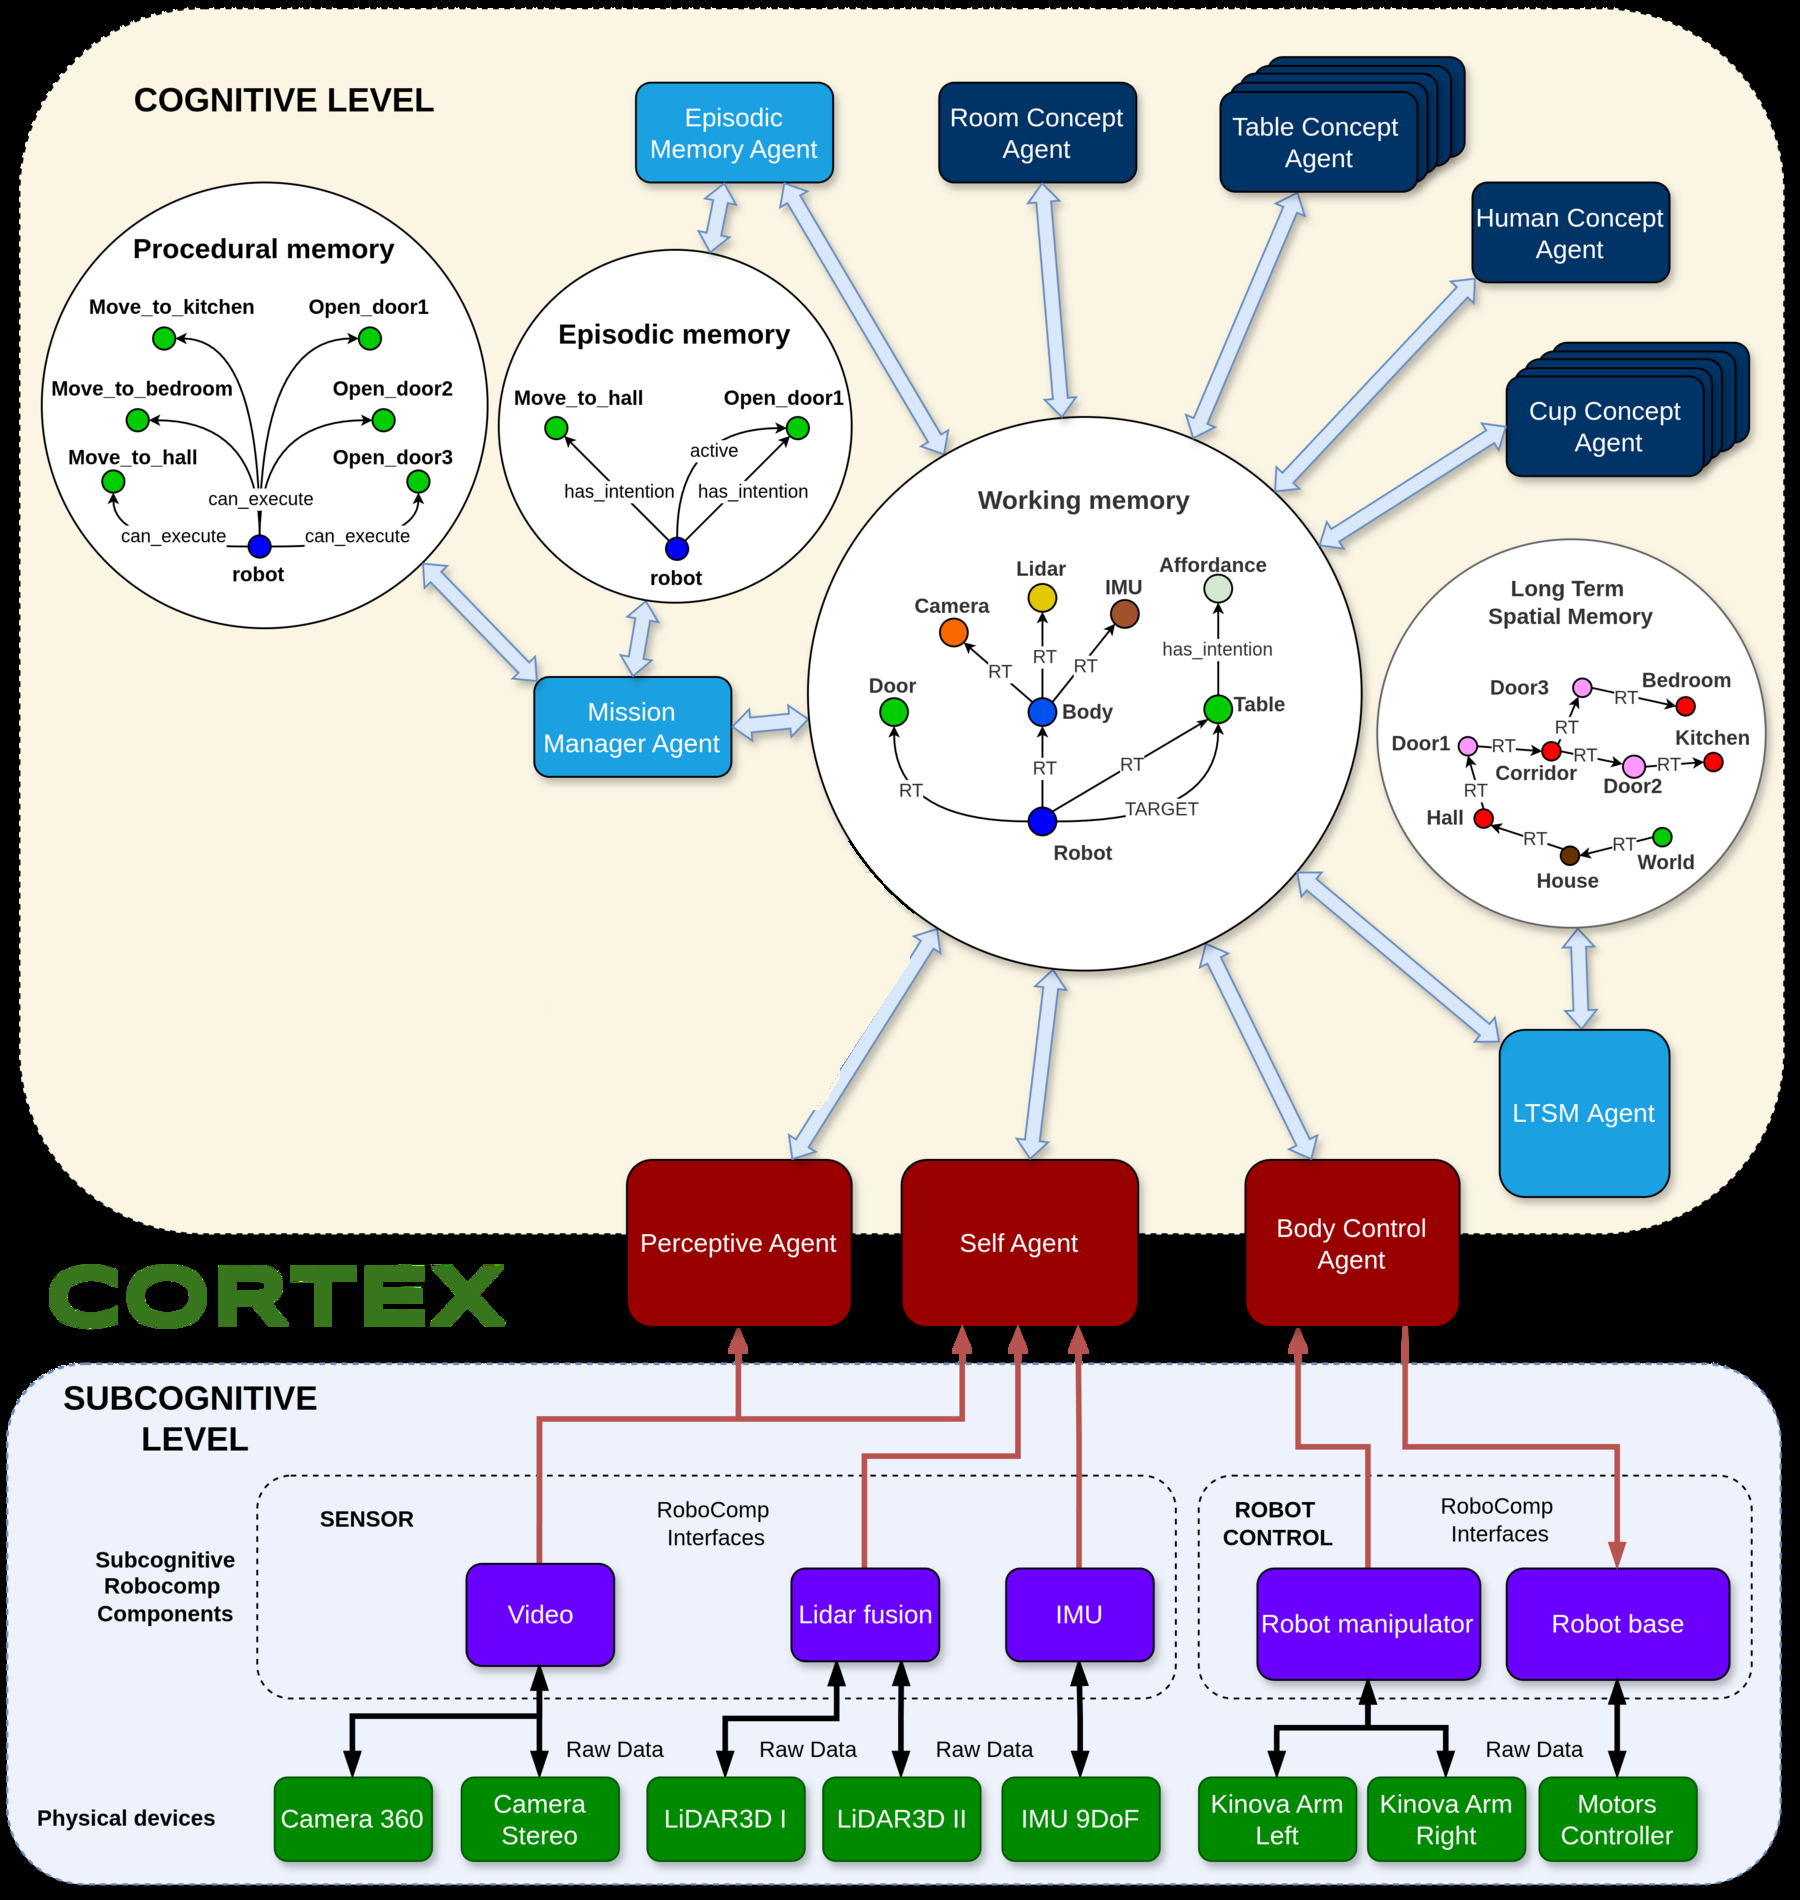
\includegraphics[height=5.6cm]{cortex_overview_nosem.png}
\end{center}

\paragraph{Why a shared graph and not messages.} \slt{Agents share a memory graph instead of sending messages to each other.} If $n$ agents talk directly, there can be $n(n-1)/2$ interfaces to agree on; if every agent talks only to the graph, there are $n$ connections. The belief is also kept in one place per piece: messages scatter it over the wires. The robot has several memories, each a graph of its own: working, episodic, long-term spatial and long-term object (Section 1.4).

\subsection{How many copies of the graph stay equal: CRDT, owners, presence}

\paragraph{Every agent keeps a full copy.} \slt{A distributed memory: each agent keeps a full copy, merged by a CRDT.} There is no server and no lock. An agent writes to its own copy and goes on; the change travels over DDS (a publish--subscribe system, explained below) as a small \emph{delta} to every other copy. A \emph{CRDT} (conflict-free replicated data type) is a data structure designed so that copies which received the same set of changes are equal, whatever the order in which they arrived and even if a change arrived twice. In CORTEX every node, every edge and every attribute is a CRDT. If two agents write the same value at the same moment, there is a tie, and the rule is that the same write wins in every copy.

\paragraph{Copies disagree for a moment.} \slt{Every agent holds a copy: copies disagree for a moment, then agree.} Take a value that is 1.0 everywhere. Agent 1 writes 2.0. Agent 2, before receiving that change, writes 2.4. Agent 3 first receives agent 2's change and believes 2.4 for a while; later the tie is resolved and every copy holds 2.0. The lesson for a programmer is that no copy may assume that the others see the same value at the same instant.

\textbf{Question on the slide:} agents 1 and 2 write the same node at once. What does agent 3 end with? \textbf{Answer:} 2.0, like every copy: the CRDT keeps one write everywhere and drops the other one. A write that is dropped is lost, which is why the architecture gives each node exactly one owner.

\paragraph{The protocol.} \slt{A protocol keeps the graph consistent: owners, presence and cleanup.} The graph accepts any write from any agent; it enforces nothing. So the agents agree on three rules, a \emph{protocol}:
\begin{enumerate}
\item \textbf{Ownership.} Only the owner of a node writes it. An agent \emph{owns} the nodes it created (\texttt{chair\_concept} owns \texttt{chair\_1}).
\item \textbf{Presence.} Every agent sends a \emph{heartbeat} each second: a small node attribute that says ``I am alive''. Other agents can then tell whether an owner is still there.
\item \textbf{Cleanup.} An agent deletes its own nodes when it stops, and at start it sweeps away the nodes that it left behind in a previous run that crashed.
\end{enumerate}
Why cleanup matters: if an agent crashes, its nodes stay in the graph and look like any other node, but nothing updates them any more; no single reader can tell this from ordinary data. Exercise 2 is exactly this problem.

\paragraph{Sensor data travels beside the graphs.} \slt{Sensor data travels beside the graphs.} The graph is small and reliable: about 1 MB/s, delivered to everyone, in DDS \emph{domain} 0. Images and LiDAR clouds are large: a 360$^\circ$ camera is about 165 MB/s, a stereo camera about 100 MB/s, a LiDAR 5 MB/s (estimates at simulator resolution, uncompressed). They go on their own channel, DDS domain 7, the \emph{media plane}, about 270 MB/s in total, where only the newest image matters. A \emph{domain} is a private channel: traffic in one domain is not seen in the other. In the working memory a node only says where each stream is.

\begin{backupbox}{Backup: \emph{On one computer: pass the place, not the image}}
Why the media plane is fast. On one computer, an image can be written once into a slot of shared memory by the driver, and every reader looks at the same bytes in place (\emph{zero copy}). Moving one 2.8 MB frame: one copy inside the computer's memory takes about $2.8\text{ MB} / 85\text{ GB/s} \approx 33\ \mu$s in theory; the measured zero-copy path takes 0.19 ms end to end (most of it is notifying and mapping, not moving bytes); 10 Gb Ethernet takes $2.8\times 8/10{,}000 \approx 2.2$ ms; 1 Gb Ethernet 22 ms. One colour+depth camera at 30 Hz is about 0.2 GB/s, a small fraction of the 80--90 GB/s the memory can move. With zero copy the cost does not grow with the number of readers; with real copies each reader pays once.
\end{backupbox}

\begin{keyidea}
CORTEX replaces messages between agents by a shared graph. Each agent keeps a full copy; a CRDT makes the copies equal; the protocol (one owner per node, heartbeat, cleanup) keeps every node with a live owner; images travel on a separate channel.
\end{keyidea}

\subsection{The working memory}

\paragraph{A graph of beliefs.} \slt{The working memory writes the scene as a graph, with the robot at the centre.} Each \emph{node} is a belief: what one agent currently thinks about one thing, with how sure it is. Each node is an \emph{instance} (this chair), owned by its concept agent. The robot is at the centre: the room hangs from it once the room is detected, and the objects hang from the room. \slt{A real working memory: the scene, the robot and the agents in one graph} shows a graph from a simulated run: the robot \texttt{Shadow} with its body and sensors; the room with chairs, a refrigerator, the floor, 33 walls and a door; offers such as \texttt{aff\_chair\_4}; and a node \texttt{mind} with the eleven running agents, each in state Operating (the agents are nodes too). Three kinds of \emph{edge} appear: \texttt{RT} (where a node is, relative to its parent), \texttt{has} (a part, or a running agent) and \texttt{has\_intention} (an offer the object makes to the robot).

\begin{backupbox}{Backup: \emph{The whole graph of a simulated run: every node has one writer}}
The same graph with every node drawn, layered by what a node is about (robot and objects, structure and places, rooms, world); colour says who wrote each node, and the bottom layer is the simulator's apartment, not a belief. Every node has one writer, as the ownership rule says.
\end{backupbox}

\paragraph{Two ways a belief changes.} \slt{A belief changes in two ways: its numbers, or its structure.} If something known moves, the numbers in its node change: data revise the belief. If the world contains something new, a node is added: the structure of the belief changes, which is a \emph{birth}. The lab calls these non-structural and structural writes. Day 4 is about births.

\paragraph{Typed attributes.} \slt{Nodes and edges are typed records of attributes.} A node has a type (\texttt{chair}), a writer, and \emph{attributes} such as \texttt{obj\_width\_m = 0.52} or \texttt{obj\_exist\_prob = 0.97}. Each attribute is stamped with its value, its time and its writer. Each attribute \emph{name} is declared once with its type, so that a wrong type is a compile error and not a crash at run time. An RT edge holds the pose of the child in the parent's frame, a covariance matrix, and a ring of past poses with their times.

\paragraph{RT edges form a tree.} \slt{The working memory is a graph; its RT edges are a tree inside it.} Every node with a place in space hangs from exactly one parent by an RT edge, back to the root. Therefore between any two such nodes there is exactly one path of RT edges, and the pose of one in the frame of the other is found by walking that path. Edges that are not RT (\texttt{close\_to}, \texttt{owns}, \ldots) do not carry poses.

\begin{center}
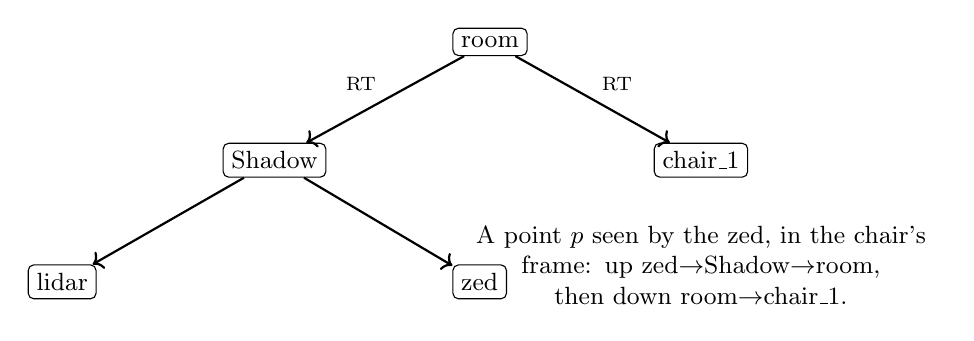
\begin{tikzpicture}[font=\small, node distance=1.1cm and 1.6cm, every node/.style={draw, rounded corners=2pt, inner sep=3pt}]
\node (room) {room};
\node[below left=of room] (sh) {Shadow};
\node[below right=of room] (ch) {chair\_1};
\node[below left=of sh] (li) {lidar};
\node[below right=of sh] (zed) {zed};
\draw[->, thick] (room)--(sh) node[midway, draw=none, above left, font=\scriptsize]{RT};
\draw[->, thick] (room)--(ch) node[midway, draw=none, above right, font=\scriptsize]{RT};
\draw[->, thick] (sh)--(li);
\draw[->, thick] (sh)--(zed);
\node[draw=none, below=0.5cm of ch, align=center, font=\small, text width=6cm] {A point $p$ seen by the zed, in the chair's frame: up zed$\to$Shadow$\to$room, then down room$\to$chair\_1.};
\end{tikzpicture}
\end{center}

\paragraph{Carrying a point, and its doubt, along the path.} \slt{The RT edges form a tree inside the working memory.} Each edge stores the child's pose in the parent's frame. Going \emph{up} an edge (child to parent) applies the stored transform $T$; going \emph{down} applies its inverse $T^{-1}$. For a point $p$ seen by the zed, the three steps are $T_{\text{Shadow}\leftarrow\text{zed}}$ (up), $T_{\text{room}\leftarrow\text{Shadow}}$ (up) and $T^{-1}_{\text{room}\leftarrow\text{chair\_1}}$ (down), and
\[
p' = T\,p,\qquad T = T^{-1}_{\text{room}\leftarrow\text{chair\_1}}\;T_{\text{room}\leftarrow\text{Shadow}}\;T_{\text{Shadow}\leftarrow\text{zed}} .
\]
The point is not exact: its depth has noise, and each transform on the path is uncertain. To carry the uncertainty through $p'=T(p)$, replace the function by its first-order expansion around the current values (a Jacobian), and add the two independent contributions:
\[
\Sigma' = J_T\,\Sigma_T\,J_T^{\top} + J_p\,\Sigma_p\,J_p^{\top}.
\]
Here $\Sigma_p$ is the covariance of $p$ itself in the zed's frame (from the depth noise of that pixel), $\Sigma_T$ is the covariance of $T$ (each edge's covariance on the path, carried to one frame and added), and $J_T$, $J_p$ are the Jacobians: how $p'$ moves when $T$ or $p$ moves by a small amount. (Each edge covariance is $6\times6$ in 3-D, and $3\times3$ in the lab's flat world: $x$, $y$, yaw.) \textbf{Question on the slide:} the robot's pose in the room becomes less sure; what happens to $\Sigma'$? \textbf{Answer:} it grows, because the edge room$\leftarrow$Shadow is on the path, so its covariance enters $\Sigma_T$.

\paragraph{Each reading with the pose it was taken at.} \slt{An RT edge keeps its last poses, each with its time.} An RT edge stores a ring of five blocks; each block has a translation, a rotation, a twist (velocity) and a time $t_k$. The next write replaces the oldest block. To get the pose at a capture time inside the ring, the translation is blended linearly and the rotation along the shortest arc (\emph{interpolation}); newer than the last block it is \emph{extrapolated} along the twist; a time outside the ring returns the end block and marks it clamped. This matters because a sensor reading is old when it arrives: a LiDAR sweep placed with the newest pose instead of its own is shifted by (pose age $\times$ speed). Each reading is paired with the pose the robot held when it was captured.

\begin{keyidea}
The working memory is one graph of beliefs. Every attribute is typed and stamped with writer and time. The RT edges form a tree of poses, so any pose is found by walking one path, and the uncertainty of every edge on the path is added to the answer. Poses are stored with their times so that a reading is placed with the pose of its own moment.
\end{keyidea}

\subsection{Concepts, the retina, and the memories}

\paragraph{A concept has four dimensions.} \slt{A concept has four dimensions, and one agent answers for all of them.} For one kind of thing (for example the chair) one agent answers for: its \emph{geometry} (where it is, what shape it has, and how sure), its \emph{life cycle} (is it still there: born, missed, forgotten, back again), its \emph{aspect} (what it looks like, how one would imagine one) and its \emph{function} (what it offers, what can be done with it). Day 4 takes the chair through all four.

\paragraph{The retina and masks.} \slt{Sensor data go through the retina, into the working memory, to the agents.} The retina is the agent that runs neural networks on the camera images and the LiDAR: it finds objects and their pixels, room surfaces and people's poses. It does not decide what exists. It writes one small \emph{mask} node per camera into the working memory. A \emph{mask} is the set of pixels of one object, with a class (\texttt{chair}), a score (0.82), and its 3-D points: from the camera's depth, or from the LiDAR hits that fall inside it. Each concept agent reads the masks of its own class, moves their points into the room frame \emph{as it was when the image was taken} (the RT ring above), and updates its objects.

\begin{center}
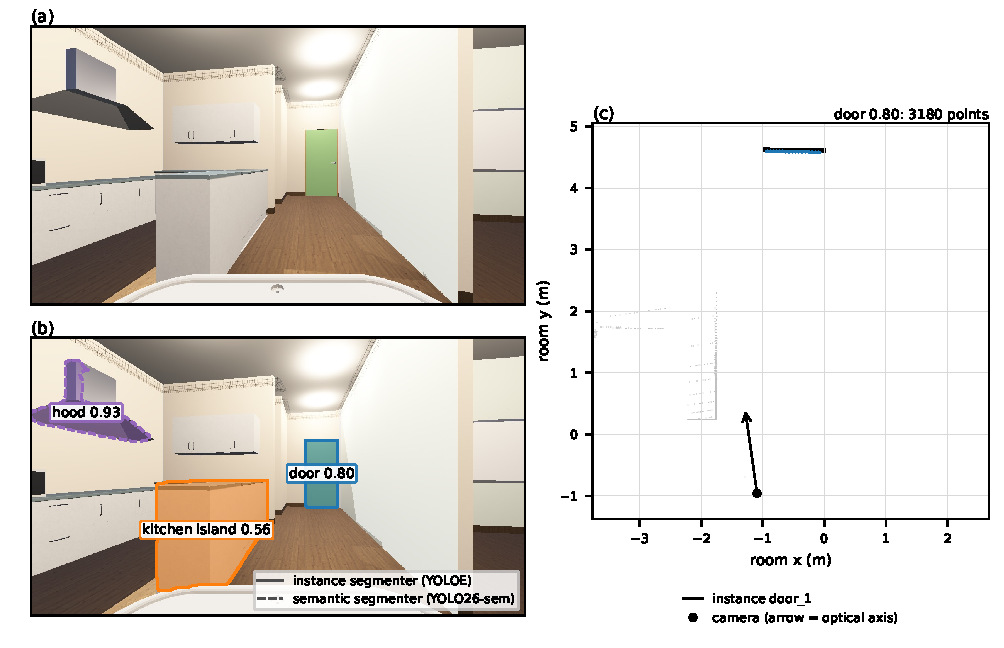
\includegraphics[height=5.2cm]{d3_mask_real.pdf}
\end{center}
\emph{Measured, simulated kitchen:} the camera image, its masks, and a top view in which the door mask's 3180 points land on the box of \texttt{door\_1}, the belief the door agent keeps.

\paragraph{A mask is evidence, not an object.} \slt{A concept agent builds one object out of many fragments.} The chair agent moves the points of its masks into the room. Points that no existing chair explains feed a \emph{provisional chair}. It is born only when its accumulated evidence $w$ reaches a fixed count. The count is a threshold, which Day 4 replaces by a quantity in nats (see the last backup slide).

\paragraph{Class and instance.} \slt{The agent holds the class. The working memory holds the instances.} The \emph{class} (what a chair is: its typical size, how it looks) lives inside \texttt{chair\_concept} as a prior. Each \emph{instance} (this chair here, that chair there) is a node in the working memory, with its own pose and its own sureness, and it is the posterior for that chair. \textbf{Question on the slide:} a third chair comes into view; what is added, an agent, a node, or both? \textbf{Answer:} one node. The agent already exists.

\paragraph{Six memories.} \slt{Memories keep the same concepts for longer.} The same concepts persist over longer times, each in a memory with an agent that fills it by watching the working memory. From shortest to longest: the \emph{working} memory (the concepts of now); the \emph{episodic} memory (what the robot undertook, and what came of it; this deployment); the \emph{long-term object} memory (this chair, again; across missions; work in progress); the \emph{long-term spatial} memory (rooms and passages); the \emph{procedural} memory (learned habits, skills; not running yet); and the \emph{semantic} memory, in two parts: the robot's own objects and common sense compiled outside (a vision-language model).

\paragraph{Episodic memory.} \slt{Episodic memory records what the robot undertook, and what came of it.} Its unit is the \emph{record}: one thing the robot undertook to do, at any level (a mission ``go to the kitchen'' contains steps ``reach the door'' and ``cross it''). A record stores what was asked, when it began and ended, the outcome its owner reported, and the target's belief before and after. Start and end are read from the controller's journal, not guessed from the world. At the turn of the day, records fold into \emph{track records}: how often crossing this door has worked, and how long it takes. \slt{One episode, as the episodic memory stores it} adds what changed while the episode lasted (here two doors appeared and one was dropped) and keeps the unrelated changes (two chairs that came and went) apart; the consequences are stored by \emph{type} (``a door''), so that what is learned holds for any door. \slt{The episodic memory as a graph} stores one node per record, hung from the root in time order, with the steps hung below the record.

\paragraph{Long-term spatial memory.} \slt{Long-term spatial memory keeps the rooms the robot has left.} The room the robot leaves moves out of the working memory and goes back in when the robot returns. The memory holds rooms and \emph{passages} only (objects now have their own memory). It plans routes across rooms and predicts a room before the robot enters it. The working memory stays small, and the map is bounded only by storage.

\paragraph{How rooms are joined.} \slt{Rooms are joined where the same door is seen from both sides.} Each room has its own frame. A door between room 1 and room 2 is seen from both rooms, so the map has two copies of it, and these must coincide. Let $X$ be the pose $(x,y,\text{yaw})$ of every room in the map and $z$ each door as seen from either side, with its covariance. The map is itself a belief, and the same free energy applies:
\[
F(X) = \underbrace{-\ln p(z\given X)}_{\text{likelihood}}\;\underbrace{-\ln p(X)}_{\text{priors}}
\]
The likelihood term is low when each door's two copies coincide. The prior term is low when rooms do not overlap, walls are square, a door's two sides lie in one wall, and joined rooms touch.
The robot computes the minimum of $F$ and its Laplace covariance (Day 2). Each door match is either an inlier (right) or an outlier (wrong); the likelihood is a mixture of the two, so a wrong match stops pulling on the solution with no threshold (see the backup on outliers below). \slt{The long-term spatial memory: three rooms, joined by passages}: after a three-room tour, the optimiser places the rooms so that the two sides of each door meet; $F$ falls from 152 to 26.

\begin{backupbox}{Backup: \emph{Long-term object memory recognises this chair, again} (work in progress)}
When the robot leaves room 1, the node \texttt{chair\_22} disappears from the working graph but is kept in a repertory: identity, class, size, its lives and how each ended, where it was last seen per room. When the robot comes back nothing appears yet; the agent compares what it sees with the repertory and \emph{offers} either the remembered identity or a new one. The memory only offers; the concept agent decides, and the object appears only when it is detected. Measured (chairs only): room 1, room 2, room 1: two chairs came back with their own identities, with belief 0.945 and 0.969 that each is the same chair. Today the comparison uses position alone; the chair's look is the missing term.
\end{backupbox}

\begin{keyidea}
The retina labels pixels; each concept agent turns the masks of its class into beliefs. The agent holds the class (a prior), the working memory holds the instances (posteriors). Memories keep the same concepts for longer and are filled by agents that watch the working memory. The map of rooms is a belief too: its likelihood comes from the doors, its priors from what buildings are like.
\end{keyidea}

\subsection{One belief, cut among many agents}

This is the central part of the day.

\paragraph{A product of factors.} \slt{The global belief q is a product of factors, each kept by one agent.} We write
\[
q(\text{everything}) \;\approx\; q(X,R)\;q(\theta_{c_1})\,q(\theta_{c_2})\,q(\theta_{t_1})\cdots
\]
with $X$ the robot's path, $R$ the room, and $\theta_{c_1},\theta_{c_2},\theta_{t_1}$ the pose and shape of \texttt{chair\_1}, \texttt{chair\_2} and \texttt{table\_1}. The first factor is held by \texttt{room\_concept}, the next two by \texttt{chair\_concept}, the last by \texttt{table\_concept}. Which mask belongs to which object is \emph{not} a factor: each agent fixes it to its best guess. Agents see each other's factors only through the graph. Day 2's single $q$ has become a product; each factor is a node that one agent keeps. The product is an \emph{assumption}: it says the pieces are independent. A line where we split $q$ is called a \emph{cut}.

\paragraph{What an agent does inside its factor.} \slt{Inside its factor, an agent estimates, reads, and guesses.} The chair agent \emph{estimates} its own factor (pose and existence of each chair, published with how sure it is). It \emph{reads} the robot's pose with its covariance from the graph: the doubt is carried along. It \emph{guesses} once which mask is which chair, keeping one best matching. The guess has no principled defence (trying every matching is impossible); a SLAM system would estimate objects and path together, as one factor.

\paragraph{Each agent lowers Day 2's $F$ for its own factor.} \slt{Each agent lowers Day 2's F for its own factor.} For object $i$,
\[
F_i(\theta_i)=\underbrace{\sum_k r_k^2/\sigma^2}_{\text{1. misfit to the masks}}\;+\;\underbrace{(\theta_i-\mu)^2/s^2}_{\text{2. distance from the class}} .
\]
Here $\theta_i$ is the object's pose and size (on the slide, the depth of a refrigerator), $r_k$ is the distance from mask point $k$ to the shape placed at $\theta_i$, $\sigma$ is one point's noise, and $\mu,s$ are the mean and spread of the depth of refrigerators, written by us. Term 1 is Day 2's accuracy (with a minus sign); term 2 is its complexity (the prior). For example, a refrigerator placed 0.80 m deep when the class mean is $\mu=0.60$ m and the spread $s=0.08$ m costs $(0.20/0.08)^2 = 6.25$ in term 2. The agent moves $\theta_i$ to lower $F_i$: with few points term 2 decides; with many points term 1 does. (The slide drops the constant $\tfrac12$ and the $\ln$ terms; the lab writes the complete version, see Exercise 5.)

\paragraph{Why the sum of the agents' $F_i$ is the global $F$ when the factors are independent.} In the lab, $n$ objects at positions $\theta_i$ are measured in $T$ frames; $z_{it}=\theta_i+\varepsilon_{it}$ with $\varepsilon_{it}\sim\N(0,r)$, and the belief is Gaussian with mean $\mu$ and covariance $\Sigma$. If the noises are independent across objects, the data covariance of one frame is $C=rI$, which is diagonal. The global free energy has a data term and a complexity term:
\begin{align*}
F&=\underbrace{\tfrac12\sum_{t}(z_t-\mu)^{\top}C^{-1}(z_t-\mu)+\tfrac T2\operatorname{tr}(C^{-1}\Sigma)+\tfrac T2\big(\ln|C|+n\ln 2\pi\big)}_{\text{data}}\\
&\quad+\underbrace{\KL{\N(\mu,\Sigma)}{\N(m_0,p_0 I)}}_{\text{complexity}} .
\end{align*}
Take $q$ with diagonal $\Sigma=\operatorname{diag}(v_i)$. Because $C^{-1}=I/r$, $\ln|C|=n\ln r$, and $\operatorname{tr}(C^{-1}\Sigma)=\sum_i v_i/r$, the data term is a sum over $i$ of $\tfrac12\sum_t[((z_{it}-\mu_i)^2+v_i)/r+\ln 2\pi r]$. The KL divergence between two Gaussians with diagonal covariances is also a sum over $i$. So $F=\sum_i F_i$ exactly, for any belief of this form, not only at the minimum. If the objects shared an error, $C$ would not be diagonal, and the sum would no longer be the whole.

\paragraph{A pose crosses the cut with its covariance.} \slt{Across a cut, a pose must travel with its covariance.} The robot's pose is the only thing the object agents read from outside. Suppose the room agent publishes a pose estimate $\hat x_t = x_t + \delta_t$ whose error $\delta_t\sim\N(0,s^2)$, and the chair agent senses the chair at relative position $\mathrm{rel}_{t}$ with noise variance $r$. The chair agent places the sighting in the room: $z_t=\hat x_t+\mathrm{rel}_t=\theta+\delta_t+\varepsilon_t$. Its error is $\delta_t+\varepsilon_t$, with variance $r+s^2$. If the agent \emph{ignores} the published covariance, it uses $R=r$; after $T$ frames, its mean has true error variance about $(r+s^2)/T$ but it claims $r/T$. The \emph{NEES} (normalised estimation error squared) is the true squared error divided by the variance the belief claims, averaged over many runs; a belief that claims the right spread has NEES $=1$. Therefore
\[
\text{NEES}\;\approx\;\frac{(r+s^2)/T}{r/T}=\frac{r+s^2}{r}=1+\frac{s^2}{r}.
\]
With the lab's numbers $r=0.05^2=0.0025\ \text{m}^2$ and $s^2=0.10^2=0.01\ \text{m}^2$ this is $1+4=5$. If the agent uses $R=r+s^2$ (the covariance added), the claim is $(r+s^2)/T$ and NEES $=1$. The lab measures 1.07 with the covariance and 5.01 without, over 2000 runs. \textbf{Question on the slide:} the robot's pose becomes exact; do the two scenes still differ? \textbf{Answer:} no; the covariance added is zero. A pose crossing a cut needs its covariance exactly when it is unsure.

\paragraph{The cost of cutting: a shared error.} \slt{The cost of cutting: one pose error moves every object together.} We write the model of one sighting of object $i$ in image $t$ as
\[
z_{it}=\underbrace{\theta_i}_{\text{where it is}}+\underbrace{\delta_t}_{\text{the robot's pose error, shared by all}}+\underbrace{\varepsilon_{it}}_{\text{its own noise}},
\]
with $\delta_t\sim\N(0,s^2)$ and $\varepsilon_{it}\sim\N(0,r)$. In one image the same $\delta_t$ shifts every object that is placed. \textbf{Question on the slide:} in one image \texttt{chair\_1} is placed 10 cm too far left; where is \texttt{table\_1} placed? \textbf{Answer:} also about 10 cm too far left, because the same $\delta_t$ moves both. In one $q$ the errors of the two objects are tilted together; the product of factors has no place for this link, so it drops it.

\paragraph{What is lost and what is kept.} Integrate $\delta_t$ out. The noise of one frame (all $n$ objects) has mean zero and covariance $C$ with entries: variance $r+s^2$ on the diagonal, and covariance $s^2$ between two different objects (they share $\delta_t$):
\[
C=r\,I+s^2\,\one\one^{\top},\qquad \one=(1,\dots,1)^{\top}.
\]
\begin{backupbox}{Backup: \emph{The shared error, as a matrix}}
$C=rI+s^2\one\one^\top$. The agents use only its diagonal, $R=r+s^2$, and drop the off-diagonal $s^2$. This is the cut, written as a matrix.
\end{backupbox}
The agent for object $i$ therefore uses $R=r+s^2$ and, over $T$ frames with a weak prior, gets the mean of its sightings with variance $(r+s^2)/T$. Compare it with the exact belief, which keeps $C$:
\begin{itemize}
\item \textbf{One object alone.} The exact standard deviation is $\sqrt{(r+s^2)/T}$, the same as the agent's: each object carries the shared error, and the agent counts it. With $T=20$: $\sqrt{0.0125/20}=2.50$ cm for both.
\item \textbf{The relation between two objects.} The difference of the two sightings in a frame is $z_{0t}-z_{1t}=\theta_0-\theta_1+\varepsilon_{0t}-\varepsilon_{1t}$: $\delta_t$ cancels. Its variance is $2r$, so the exact standard deviation of $\theta_0-\theta_1$ is $\sqrt{2r/T}=\sqrt{2\cdot0.0025/20}=1.58$ cm. Two independent agent beliefs can only add their variances: $\sqrt{2(r+s^2)/T}=\sqrt{2\cdot 0.0125/20}=3.54$ cm, more than twice as large.
\end{itemize}
This is why the robot can know how far the bottle is from the table much better than where either one is: the pose error is common to both, and it cancels in the difference. The product of factors cannot say that.

\paragraph{The price of the cut, in nats.} The price is $\KL{q}{p(\theta\given z)}$, where $q$ is the product of the agents' beliefs and $p(\theta\given z)$ is the exact posterior. By Day 2's identity $F(q)=\KL{q}{p(\theta\given z)}-\ln p(z)$, the price also equals $F(q)-F(\text{exact})$ in nats, because $-\ln p(z)$ is the same for both. For two Gaussians with a weak prior and many frames, $q=\N(\mu,\tfrac{r+s^2}{T}I)$ against $\N(\mu,\tfrac1T C)$, and with $a=s^2/r$, the eigenvalues of $C$ are $r$ (multiplicity $n-1$) and $r(1+na)$, so
\[
\text{price}=\tfrac12\Big[(1+a)\Big(n-1+\tfrac1{1+na}\Big)-n+\ln\frac{1+na}{(1+a)^n}\Big].
\]
This depends on $a=s^2/r$ and on $n$ only; the number of frames $T$ cancels. For $a=4$: $n=2$: 1.27 nats; $n=5$: 5.12; $n=10$: 11.37. These match the lab (Exercise 7).

\begin{keyidea}
$q$ becomes a product of factors, one per agent. Each agent lowers its own $F_i$ (accuracy + complexity on its own sightings). If nothing couples the pieces, $\sum_i F_i$ is exactly the global $F$. A pose crossing a cut must carry its covariance, or the receiver is overconfident by $(r+s^2)/r$. What the cut loses is the correlation between objects: each object alone is right, but the relation between two objects is estimated much less sharply than the exact belief allows, at a price in nats that grows with $s^2/r$ and with $n$ and does not fall with more frames.
\end{keyidea}

\subsection{No thresholds, and the one that stays}

\paragraph{Why not a threshold.} The modelling rule of this project: do not add a threshold if the effect can be written in the generative model. A threshold is a number tuned to one scene; a \emph{precision} that follows the physics is part of the model and is written once. \slt{Replace a threshold by a precision that follows the physics.} Three physical facts, each a variance and not a switch: far away the robot is less sure about direction; when the robot moves, the image is blurred, so the variance is larger; many points on one object share one error, so they stop helping each other. A threshold such as ``ignore anything beyond 5 m'' throws away a sighting at 5.1 m. A precision uses it, with weight $1/\sigma(\rho)^2$, where $\sigma(\rho)$ is the noise at range $\rho$. With the lab's $\sigma(\rho)=0.02(1+(\rho/2)^2)$ m: $\sigma(4.9)=0.140$ m and $\sigma(5.1)=0.150$ m, so the sighting at 5.1 m weighs $(0.140/0.150)^2\approx0.87$ of the one at 4.9 m: a little less, not zero. \textbf{Question on the slide:} a chair is seen at 5.1 m; what does each version do with it? \textbf{Answer:} the threshold throws it away; the precision uses it, with a little less weight than at 4.9 m.

\paragraph{A tuned threshold fails on the next pass.} \slt{A tuned threshold fails on the next pass; a sensor model does not.} The robot drives from $-8$ to $8$ m along a line, $\ell$ metres from an object, and measures $\ell$ at 41 equally spaced points with noise $\sigma(\rho)$, $\rho=\sqrt{x^2+\ell^2}$. The \emph{threshold} estimator averages the sightings with $\rho<k$. On a near pass ($\ell=1$ m) the best value is $k=2$ m with rmse 1.01 cm (the curve is U-shaped: small $k$ throws away useful sightings; large $k$ admits far sightings that are much noisier but count the same). Use the same $k=2$ m on a far pass ($\ell=6$ m): every sighting has $\rho\ge6>k$, so none is admitted, and the estimator returns its prior guess, 3.0 m, which is 300 cm off. The best threshold of the far pass is 8 m (rmse 4.79 cm). The \emph{precision} estimator, weights $1/\sigma(\rho)^2$, needs no tuning and gets 0.86 cm (near) and 4.22 cm (far), below the best threshold of each pass.

\paragraph{A threshold that stays.} \slt{One threshold stays: a bias the per-frame model has no place for.} A variance handles an error that averages out over frames. A \emph{bias} $b$ shared by consecutive frames does not: frames taken while the robot moves fast are all smeared the same way. Let the prior have precision $\Lambda_0$, each frame precision $\Lambda$ multiplied by an attenuation $\alpha\in[0,1]$ (1 means fully counted; 0 means ignored), and let every frame, on average, read the truth plus $b$. The precision-weighted mean after $n$ frames is
\[
\Delta\mu_n=\frac{n\alpha\Lambda}{\Lambda_0+n\alpha\Lambda}\;b .
\]
Derivation: the posterior precision is $\Lambda_0+n\alpha\Lambda$; the posterior mean is the precision-weighted average of the prior mean (the truth, taken as 0) and $n$ readings equal to $b$, which gives the formula. For any $\alpha>0$ the fraction tends to 1 when $n$ grows, so the mean ends displaced by the \emph{whole} bias. Down-weighting changes how fast it gets there (about $n\approx\Lambda_0/(\alpha\Lambda)$ frames for half of it) and not where it ends. Only $\alpha=0$, ignoring those frames (a threshold), keeps the displacement at 0. So the rule is not ``never a threshold'' but ``declare it and justify it'': the justification here is that the model has no coordinate for a bias shared across frames.

\begin{backupbox}{Backup: \emph{An outlier costs a bounded amount, and nobody rejects it}}
Under least squares a point's cost grows with the square of its residual, so one wrong point can pull the estimate far. A rejection rule (a cliff) removes points beyond a cutoff: it is a threshold. A \emph{mixture} gives every point three possible explanations: the object, clutter, or a known wall. A point that fits none costs a finite amount and stops pulling on the estimate. Nobody decided to reject it; the bound is a probability in the model.
\end{backupbox}

\begin{backupbox}{Backup: \emph{The rule is: declare it, justify it, or remove it}}
Three examples from the real system. (1) Ignoring a bad frame stays: no per-frame precision can bound a shared bias (the section above). (2) Birth after $N$ sightings must go: a count standing in for nats. (3) Waiting a few seconds for a peer is a debt: whether a peer is alive is a belief too. Measured: a test that used the agent's own estimate (a chair's ``can I see its yaw?'' was computed from its own yaw; the yaw was about $45^\circ$ wrong, so the test said no, and the wrong yaw froze).
\end{backupbox}

\begin{backupbox}{Backup: \emph{The whole scene, in causal order} and \emph{from the exact posterior to what actually runs}}
The full generative model, in the order things happen: objects exist and have a shape ($P(\ell)P(\theta\given\ell)$, with $\ell$ the labels and $\theta$ the geometry; the object agents); the room has walls, the robot moves, the wheels report it, the LiDAR hits it all ($P(R)P(X)P(\Phi\given X)P(L\given X,R,\theta)$; the room agent); what is visible from where ($P(M\given\theta,\ell,X)$, $M$ the matching); surfaces become masks ($P(Z\given\theta,M,X)$). Objects and pose are independent a priori, but once data arrive they are coupled twice: through the masks, and through the LiDAR sweep, which hits the fridge as well as the wall behind it. What runs differs from the exact posterior by seven assumptions, each with a justification and a cost: A1 objects as landmarks; A2 the pose error is integrated per frame (this is $\Sigma_t^\delta$, the covariance added above); A3 hard matching ($\mathbf 1[M=\hat M]$, the single best guess); A4 classes apart; A5 instances apart; A6 geometry and existence apart; A7 Markov time.
\end{backupbox}

\begin{keyidea}
Write the effect as a precision that follows the physics (range, motion, shared error) and nothing is tuned to one scene. Down-weighting cannot remove a bias shared by many frames, because for any $\alpha>0$ the displacement tends to the whole $b$; that is the one threshold that stays, and it must be declared and justified.
\end{keyidea}

\paragraph{Tomorrow.} The same $F$ builds the room and the chair (their births, misses and forgetting are terms of $F$), and the expected free energy $G$ chooses where to look. Reading for Day 4: the thesis chapters \emph{The Life Cycle of a Concept Agent} and \emph{The Room Concept Agent and Robot Localisation}.

%=====================================================================================
\section{Lab guide}
%=====================================================================================

The notebook is \texttt{labs/day3.ipynb}; the orange lines are the numbers you should find. \textbf{In class:} Exercises 3, 4, 5, 6 and 8 (about 55 minutes). \textbf{At home:} 1, 2, 7 and 9. The notebook defines the toy \texttt{Graph} (from \texttt{toyworld}); only the pieces you need are below.

\begin{labhelp}{The toy \texttt{Graph}: what you can call}
\texttt{g.add\_node(name, type, parent=, pose=, cov=, owner=, **attrs)} returns the node id and creates the RT edge to \texttt{parent}. \texttt{g.node(key)} returns the \texttt{Node} for a name \emph{or} an id; it has \texttt{.id}, \texttt{.name}, \texttt{.type}, \texttt{.owner}, \texttt{.attrs} (a dict). \texttt{g.update(key, **attrs)} changes attributes. \texttt{g.remove(key)} removes a node \emph{and its whole subtree}. \texttt{g.nodes} is a dict id $\to$ node. \texttt{g.by\_type(t)} lists nodes of a type. \texttt{g.rt[child\_id]} is \texttt{(parent\_id, RT)} with \texttt{RT.pose} and \texttt{RT.cov} ($3\times3$). \texttt{g.transform(dst, src)} gives the pose of \texttt{src} in the frame of \texttt{dst}: name two frames and ask the graph. \texttt{OwnedGraph} (Exercise 1) adds the owner check and a \texttt{log}.
\end{labhelp}

\subsection*{Section 1: the shared graph (homework). Slides: \emph{A protocol keeps the graph consistent}; \emph{Every agent holds a copy}}

\begin{labhelp}{Exercise 1 (homework): ownership}
\textbf{Goal.} Make ``one process per factor'' true at run time: only a node's owner may write or delete it. \textbf{Steps.} In \texttt{write}: get the node with \texttt{self.node(key)}; if \texttt{n.owner != writer} raise \texttt{PermissionError} with a message; otherwise call \texttt{self.update(key, **attrs)} and append \texttt{("non-structural", writer, n.name)} to \texttt{self.log}. In \texttt{delete}: same check; keep \texttt{n.name} \emph{before} calling \texttt{self.remove(key)}; log \texttt{("structural", writer, name)}. \textbf{Check.} The bottle agent's write to \texttt{table\_1} prints \texttt{refused: bottle\_concept may not write table\_1, owned by table\_concept}; the table keeps $\mu=2.02$; the log has three structural creates and one non-structural write; \texttt{g.transform("table\_1","bottle\_1")} is $[0.1,\,0.1,\,0]$. \textbf{Common mistakes.} Logging before the owner check (a refused call must leave no log entry); reading \texttt{n.name} after \texttt{remove}; checking the owner of the wrong node.
\end{labhelp}

\begin{labhelp}{Exercise 2 (homework): a factor nothing is minimising}
\textbf{Goal.} After a crash the dead agent's node stays and looks like any data. Write \texttt{sweep(g, alive)} that removes every node whose owner is not in \texttt{alive}, and returns the removed names. \textbf{Steps.} Loop over \texttt{list(g.nodes.values())} (a \emph{copy}: you remove while looping); skip nodes with an empty owner (the root); for a dead owner append the name and call \texttt{g.remove(n.id)}. \textbf{Careful.} \texttt{remove} deletes the subtree, so a later node of the list may already be gone: test \texttt{n.id in g.nodes} first. \textbf{Check.} With \texttt{alive=\{"room\_concept","table\_concept"\}} the result is \texttt{['bottle\_1']} and only \texttt{table\_1} remains of type object. \textbf{Think.} What would happen to a live agent's node hanging below a dead agent's node? (It is removed too; the real protocol avoids this by letting each agent decide.)
\end{labhelp}

\subsection*{Section 2: agents that only read and write (in class, 15 min). Slide: \emph{Across a cut, a pose must travel with its covariance}}

\begin{labhelp}{Exercise 3 (in class): the object agent}
\textbf{Goal.} An object agent reads the robot's pose from the graph, forms $z=\hat x+\mathrm{rel}$, and updates its belief with Day 2's rule (precisions add). It never calls the localiser. \textbf{Formulas.}
\[
R=\begin{cases}r+s^2 & \text{use\_cov}\\ r & \text{otherwise}\end{cases},\quad
\Lambda_{\text{new}}=\frac1{\text{var}}+\frac1R,\quad
\mu_{\text{new}}=\frac{\mu/\text{var}+z/R}{\Lambda_{\text{new}}},\quad \text{var}_{\text{new}}=\frac1{\Lambda_{\text{new}}}.
\]
\textbf{Code.} \texttt{x\_hat, var\_x = robot\_belief(self.g)} returns the published pose and variance along $x$ (read them, do not use the true pose; the agent does not know it). The old belief is in \texttt{attrs["mu"]}, \texttt{attrs["var"]}. Write the result with \texttt{self.g.write(self.owner, self.node, mu=..., var=...)}: the writer must be the agent's \emph{own} owner string, or Exercise 1 refuses it. \textbf{Check.} One run prints published means near $[1.04,\,2.52,\,4.03]$ (true $[1,2.5,4]$) and all three standard deviations $0.025$. \textbf{Common mistakes.} Using \texttt{self.r} for $R$ always; forgetting that \texttt{var} is a variance and not a standard deviation; overwriting \texttt{attrs} instead of passing the new values to \texttt{write}.
\end{labhelp}

\begin{labhelp}{Exercise 4 (in class): is the published covariance needed?}
\textbf{Goal.} Measure the mean NEES with and without the covariance. \textbf{Steps.} Repeat \texttt{run\_trial(rng, use\_cov)} 2000 times; each call returns arrays \texttt{mu}, \texttt{var} of length 3; collect \texttt{(mu - THETA)**2 / var} and average over both runs and objects. \textbf{Before you run, predict:} the claim is $r/T$ and the truth $(r+s^2)/T$, so NEES $\approx (r+s^2)/r=5$ (see Section~1.5). \textbf{Check.} 1.07 with the covariance, 5.01 without; the notebook prints the prediction 5.00. Small differences from 5.00 are sampling noise. \textbf{Common mistakes.} Averaging $\mu-\theta$ (the sign cancels) and not its square; dividing by the standard deviation instead of the variance.
\end{labhelp}

\subsection*{Section 3: one free energy, many owners (in class; Exercise 7 at home). Slides: \emph{The global belief q is a product of factors}; \emph{Each agent lowers Day 2's F}; \emph{The cost of cutting}}

\begin{labhelp}{Exercise 5 (in class): write the agent's free energy}
\textbf{Goal.} Code $F_i$ and check that, with no shared error ($s^2=0$), $\sum_iF_i$ equals the global $F$ for \emph{any} belief. \textbf{Formula} (\texttt{z\_i} has shape \texttt{(frames,)}, \texttt{R} is a number):
\[
F_i(\mu_i,v_i)=\sum_t\tfrac12\Big[\frac{(z_{it}-\mu_i)^2+v_i}{R}+\ln 2\pi R\Big]+\KL{\N(\mu_i,v_i)}{\N(m_0,p_0)} .
\]
\textbf{Code.} \texttt{0.5 * np.sum(((z\_i - mu\_i)**2 + v\_i)/R + np.log(2*np.pi*R))} plus \texttt{kl\_gauss\_diag(mu\_i, v\_i, m0, p0)}, which the notebook gives you. Note $v_i$ is added \emph{inside} the sum, once per frame. \textbf{Check.} The two printed numbers agree to six digits: 416.839925 (the exact value depends on the random draw, but the two must agree). \textbf{Why it works:} the derivation in Section~1.5, paragraph ``Why the sum\ldots''. \textbf{Common mistakes.} Using $\ln R$ and not $\ln 2\pi R$; dropping the KL term; using \texttt{np.mean} instead of \texttt{np.sum} over the frames.
\end{labhelp}

\begin{labhelp}{Exercise 6 (in class): what is right and what is wrong}
\textbf{Goal.} Minimise each $F_i$ and compare with the exact posterior (the notebook's \texttt{exact\_posterior}). \textbf{Formulas.} Setting $\partial F_i/\partial\mu_i=0$ and $\partial F_i/\partial v_i=0$, with $R=r+s^2$ and $T$ frames:
\[
\Lambda=\frac1{p_0}+\frac TR,\qquad \mu_i=\frac{m_0/p_0+\sum_t z_{it}/R}{\Lambda},\qquad v_i=\frac1\Lambda .
\]
\textbf{Code.} \texttt{agent\_optimum} returns two arrays of length $n$: \texttt{z.sum(axis=0)} sums over frames (shape \texttt{(n,)}), and \texttt{np.full(z.shape[1], 1.0/info)} for the variances. \textbf{Check.} One object: exact sd 2.50 cm, agent sd 2.50 cm. The relation $\theta_0-\theta_1$: exact 1.58 cm, agents 3.54 cm (for agents, variances of two independent beliefs add: \texttt{v\_a[0]+v\_a[1]}; the exact one uses $\Sigma_{00}+\Sigma_{11}-2\Sigma_{01}$). \textbf{Explain} in one sentence why the exact relation is sharper (the shared error cancels in the difference, Section~1.5). \textbf{Common mistakes.} Using $r$ and not $r+s^2$ in the agent; forgetting that the covariance term $-2\Sigma_{01}$ is what the agents cannot have.
\end{labhelp}

\begin{labhelp}{Exercise 7 (homework): the price of the boundary, in nats}
\textbf{Goal.} Show that the price is the KL and the difference of global free energies, then see how it depends on $s^2/r$ and $n$. \textbf{Code} in \texttt{price}: get \texttt{exact\_posterior} and \texttt{agent\_optimum} for $s^2=\text{ratio}\cdot r$, then \texttt{kl\_gauss(mu\_a, np.diag(v\_a), mu\_x, Sig\_x)} (the agents' belief is the first argument: the KL has an order). \textbf{Check.} $\text{KL}=2.5606$ nats equals $F(\text{agents})-F(\text{exact})=2.5606$ nats (the assertion passes, \texttt{atol=1e-6}). At $s^2/r=4$: $n=2,5,10\to 1.27,\ 5.12,\ 11.37$ nats; 3 objects with 10/40/160 frames $\to 2.56,\ 2.56,\ 2.56$. \textbf{Answer.} The price grows with $s^2/r$ and with $n$ and does not depend on the number of frames: more data sharpens each belief, but cannot restore a correlation the product has no place to hold. You can also check your curve against the closed formula in Section~1.5. \textbf{Common mistake.} Swapping the arguments of the KL.
\end{labhelp}

\subsection*{Section 4: no thresholds (in class, 15 min). Slides: \emph{Replace a threshold by a precision}; \emph{A tuned threshold fails on the next pass}}

\begin{labhelp}{Exercise 8 (in class): a range threshold against a precision}
\textbf{Goal.} Complete two estimators for the sightings array \texttt{y} of shape \texttt{(trials, 41)} (one row per simulated pass) and the ranges \texttt{rho} of shape \texttt{(41,)}. \textbf{\texttt{gated}:} the mean of the sightings with $\rho<k$, or the prior guess 3.0 when none qualifies. Key lines: \texttt{m = rho < k} (a boolean vector over the 41 columns), \texttt{y[:, m].mean(axis=1)} if \texttt{m.any()}, else \texttt{np.full(len(y), prior)}. \textbf{\texttt{weighted}:} $\hat\ell=\sum_t w_ty_t/\sum_tw_t$ with $w_t=1/\sigma(\rho_t)^2$: \texttt{w = 1/sig\_range(rho)**2}, \texttt{(y*w).sum(axis=1)/w.sum()}; \texttt{y*w} broadcasts the weights over the rows. \textbf{Check.} Lateral 1 m: best threshold 2.25 m, rmse 1.02 cm; precision 0.84 cm. Lateral 6 m: best threshold 8.25 m, rmse 4.78 cm; precision 4.20 cm (the slide's figure comes from another run: 2 m, 1.01, 0.86, 4.79, 4.22). The threshold tuned on the near pass, used on the far pass: rmse 300.0 cm. \textbf{Answer the three questions of the notebook:} (1) the U shape: small $k$ discards useful sightings, large $k$ admits noisier ones that count the same. (2) No threshold can be shipped: the best of one scene returns nothing on the other. (3) \texttt{weighted} needs $\sigma(\rho)$, a model of how the sensor degrades; it fails if that model is wrong, but then the NEES test of lab section 2 can detect it, which a threshold does not allow. \textbf{Common mistakes.} Using \texttt{<=} and not \texttt{<} (no practical difference here, but keep the slide's definition); taking \texttt{1/sig\_range(rho)} without squaring.
\end{labhelp}

\subsection*{Section 5: the threshold that stays (homework). Slide: \emph{One threshold stays}}

\begin{labhelp}{Exercise 9 (homework): displacement by a shared bias}
\textbf{Goal.} Code $\Delta\mu_n=\dfrac{n\alpha\Lambda}{\Lambda_0+n\alpha\Lambda}\,b$ and check it against the recursive update. \textbf{Constants.} $\Lambda_0=1/0.10^2=100$, $\Lambda=1/0.05^2=400$, $b=0.03$ m. \textbf{Code.} One line: \texttt{n*alpha*lam/(lam0 + n*alpha*lam) * b}; it works on arrays \texttt{n}. \textbf{Check.} The assertions compare it with \texttt{recursive(200, a)} for $\alpha=1,0.3,0.05$. At $n=2000$ frames the displacement in cm is: $\alpha=1$: 3.0; $0.3$: 3.0; $0.05$: 2.99; $0$: 0.0. \textbf{Answer.} Attenuation changes the rate (the curve moves right by about $1/\alpha$) and not the limit: for every $\alpha>0$ the mean ends displaced by the whole $b=3$ cm; only $\alpha=0$ bounds it. \textbf{Common mistake.} Expecting a small $\alpha$ to give a small final displacement: it only delays it.
\end{labhelp}

%=====================================================================================
\section{Glossary}
%=====================================================================================

Each entry has a plain definition and the slide where the word first appears (slide titles are shortened; ``Lab'' is the lab slide).

\small
\setlength{\LTpre}{2pt}\setlength{\LTpost}{2pt}
\renewcommand{\arraystretch}{1.12}
\begin{longtable}{@{}>{\raggedright\bfseries}p{2.8cm} p{8.9cm} >{\raggedright\arraybackslash}p{4.2cm}@{}}
\toprule
Term & Meaning & Slide\\\midrule\endhead
\multicolumn{3}{@{}l}{\emph{The graph and its parts}}\\
node & One belief in the graph: what one agent currently thinks about one thing, with how sure it is. It has a type, an owner and attributes. & The working memory is a graph; its RT edges are a tree\\
edge & A link between two nodes. It has a type (\texttt{RT}, \texttt{has}, \texttt{owns}, \texttt{has\_intention}, \texttt{close\_to}, \ldots). & A real working memory\\
attribute & A named value on a node or edge, with a declared type, a time and a writer (for example \texttt{obj\_width\_m = 0.52}). & Nodes and edges are typed records of attributes\\
RT edge & An edge that holds the pose of the child node in its parent's frame, with a covariance and a ring of past poses. The RT edges alone form a tree. & The RT edges form a tree\\
frame & A coordinate system attached to a node (the room, the robot, a sensor). A pose is always a pose in some frame. & The RT edges form a tree\\
pose, covariance & Position and orientation of one frame in another; the covariance is the matrix of how unsure each part is ($3\times3$ in the lab's flat world, $6\times6$ in 3-D). & The RT edges form a tree\\
ring of poses & The last five poses of an RT edge with their times; it allows a reading to be paired with the pose of its capture time (interpolation or extrapolation). & An RT edge keeps its last poses\\
twist & The velocity stored with a pose, used to extrapolate beyond the last stored time. & An RT edge keeps its last poses\\
working memory & The robot's current state as one graph: the scene, the robot, its offers and the agents. Each agent keeps a full copy. & CORTEX: memories as graphs\\
instance & One particular thing, such as \texttt{chair\_22}: a node in the working memory with its own pose and sureness (a posterior). & The agent holds the class\\
class & What a kind of thing is like (what a chair is): a prior held inside the concept agent. & The agent holds the class\\
mask & The set of pixels of one object found by the retina, with a class, a score and 3-D points. It is evidence, not an object. & Sensor data go through the retina\\
retina & The agent that runs neural networks on the camera images and LiDAR and writes masks (and room surfaces and people's poses) into the graph. It labels pixels and decides nothing about what exists. & Sensor data go through the retina\\
birth & The addition of a new node: a structural change of the belief, as opposed to a change in numbers. & A belief changes in two ways\\
provisional object & A candidate object that collects evidence; it is born when its evidence $w$ reaches a count (a threshold that Day 4 replaces). & A concept agent builds one object out of many fragments\\
\midrule
\multicolumn{3}{@{}l}{\emph{Agents}}\\
agent & One process of the robot's software that reads and writes the shared graph; it never messages another agent. Factor, owner and writer are roles of an agent. & CORTEX: memories as graphs\\
concept agent & An agent responsible for one kind of thing (chair, door, room): one class, one belief; it answers for geometry, life cycle, aspect and function. & A concept has four dimensions\\
memory agent & An agent that fills one memory by watching the working memory (episodic, long-term spatial, long-term object). & Memories keep the same concepts for longer\\
component & A RoboComp program that reaches the robot's body or sensors (a driver). & CORTEX: memories as graphs\\
owner / writer & The one agent that may change a node. Two writes to one value cannot both survive, so every node has one owner. & Every agent holds a copy; A protocol keeps the graph consistent\\
factor & One piece of the global belief, kept by one agent: $q=\prod_i q_i$. & The global belief q is a product of factors\\
cut & A place where the belief is split into factors. Whatever correlates the two sides is dropped there, and what crosses must carry its covariance. & Across a cut, a pose must travel with its covariance\\
\midrule
\multicolumn{3}{@{}l}{\emph{Distribution and protocol}}\\
CRDT & Conflict-free replicated data type: a structure whose copies end equal when they have received the same changes, in any order and even repeated. Every node, edge and attribute is one. & A distributed memory\\
delta & The small description of one change that travels to every copy. & A distributed memory\\
DDS & Data Distribution Service: a publish--subscribe system. A writer publishes on a topic; every subscriber to that topic receives it. No server. & A distributed memory\\
domain & A private DDS channel. Domain 0 carries the graphs; domain 7 carries sensor data. & Sensor data travels beside the graphs\\
media plane & The separate DDS domain for large sensor streams (images, point clouds), where only the newest matters and readers share memory without copying. & Sensor data travels beside the graphs\\
zero copy & A reader looks at the bytes the driver wrote, in place; the cost does not grow with the number of readers. & Backup: On one computer\\
protocol & The three rules all agents agree on, because the graph accepts any write: ownership, presence, cleanup. & A protocol keeps the graph consistent\\
presence, heartbeat & Each agent publishes a small ``alive'' signal each second; others read it to know the owner is there. & A protocol keeps the graph consistent\\
cleanup, sweep & Deleting one's own nodes on stop, and at start removing the nodes left by a previous crashed run. & A protocol keeps the graph consistent\\
\midrule
\multicolumn{3}{@{}l}{\emph{Memories}}\\
episodic memory & Records of what the robot undertook (mission, steps), with the outcome and the target's belief before and after; folded into track records. & Episodic memory records\ldots\\
long-term spatial memory & Rooms the robot has left and the passages between them; plans routes across rooms. & Long-term spatial memory keeps\ldots\\
long-term object memory & Remembers identities of objects across missions (this chair, again); only offers, the concept agent decides. Work in progress. & Backup: Long-term object memory\\
procedural memory & Learned habits and skills; not running yet. & Memories keep the same concepts for longer\\
semantic memory & Knowledge about the world: the robot's own objects, and common sense compiled outside by a vision-language model. & Memories keep the same concepts for longer\\
record, episode & One thing the robot undertook, as stored in the episodic memory. & One episode, as the episodic memory stores it\\
passage & A node of the spatial memory that joins a door seen from one room to the same door seen from the other. & Rooms are joined where the same door is seen from both sides\\
\midrule
\multicolumn{3}{@{}l}{\emph{Inference terms}}\\
precision & One over the variance. Independent precisions add; a precision that falls with range down-weights far sightings continuously. & Replace a threshold by a precision\\
threshold & A hard cutoff (``ignore beyond 5 m''), tuned to one scene. The project avoids it unless it is declared and justified. & Replace a threshold by a precision\\
NEES & Normalised estimation error squared: true squared error divided by the variance the belief claims. It is 1 when the claim is right, above 1 when the belief is overconfident. & Across a cut, a pose must travel with its covariance\\
common-mode (shared) error & An error that appears equally in many measurements (here, the robot's pose error $\delta_t$ in one image, or a bias over many frames). It does not average out over the objects or frames that share it. & The cost of cutting; One threshold stays\\
bias & A systematic error shared by many frames; down-weighting those frames changes the speed, not the limit, of its effect. & One threshold stays\\
attenuation $\alpha$ & A factor in $[0,1]$ that multiplies a frame's precision; $\alpha=0$ ignores the frame. & One threshold stays\\
Laplace covariance & The covariance of a Gaussian fitted at the minimum of $F$, from the curvature there (Day 2). & Rooms are joined where the same door is seen\ldots\\
inlier, outlier, mixture & An inlier is a correct match, an outlier a wrong one; a mixture likelihood allows both, so a wrong match has a bounded cost. & Rooms are joined\ldots; Backup: An outlier costs a bounded amount\\
price of the cut & $\KL{q}{p(\theta\given z)}$ in nats for the product $q$ of the agents' beliefs against the exact posterior. & Lab 3 (Exercise 7)\\
\bottomrule
\end{longtable}

\end{document}
